\documentclass[11pt,twocolumn]{article}
\usepackage[a4paper,margin=1.85cm,columnsep=0.7cm]{geometry}
\usepackage{amsmath,amssymb,booktabs,graphicx,microtype}
\usepackage[hidelinks]{hyperref}
\usepackage{xcolor}
\usepackage{enumitem}
\usepackage{caption}

\graphicspath{{../results/figures/}}
\captionsetup{font=small,labelfont=bf}
\setlength{\parindent}{1em}
\setlength{\parskip}{0.15em}
\setlength{\tabcolsep}{3pt}
\setlist{nosep,leftmargin=*}
\newcommand{\pct}[1]{#1\%}

\title{\vspace{-1.2cm}\textbf{Comparing AMM Mechanisms:}\\
Slippage, Impermanent Loss, and Deterministic LP Returns}
\author{BitDA Final Project}
\date{June 2026}

\begin{document}
\maketitle

\begin{abstract}
Automated market makers (AMMs) exchange simplicity, capital efficiency, and
portfolio exposure in materially different ways. This study implements a
reproducible analytical simulator for four designs: Uniswap V2 constant
product, Uniswap V3 fixed-range concentrated liquidity, Curve StableSwap, and
Balancer weighted pools. We compare nine configurations over three liquidity
levels, seven normalized trade sizes, six terminal price changes, and three
fixed daily-volume assumptions. StableSwap with amplification $A=1000$
produces only \pct{0.061} slippage for a trade equal to \pct{10} of total value
locked (TVL), while Uniswap V2 produces \pct{16.875}. However, high
amplification increases loss during a small depeg. Narrow Uniswap V3 liquidity
also minimizes slippage, but its fixed range produces the greatest loss after
large price moves. Balancer's 80/20 pool has worse slippage in the tested trade
direction but lower impermanent loss than a 50/50 pool. The results show that
AMM selection is a market-design decision rather than a universal ranking.
\end{abstract}

\section{Introduction}

An AMM replaces an order book with an invariant that determines how pool
inventory and price change after a trade. The invariant makes execution
available without a matching counterparty, but liquidity providers (LPs)
implicitly sell assets that appreciate and buy assets that depreciate.
Different AMMs control this inventory response differently. Constant-product
pools are general and permissionless; concentrated liquidity allocates capital
to a selected price interval; StableSwap flattens the price curve for
correlated assets; and weighted pools encode asymmetric portfolio exposure.

This report answers three questions:
\begin{enumerate}
  \item How do the mathematical mechanisms change execution slippage?
  \item How do terminal prices change LP value relative to holding?
  \item Under fixed 30-day volume assumptions, when do fees compensate for
  impermanent loss?
\end{enumerate}

The contribution is a small, tested simulator rather than a qualitative
comparison alone. Every reported result is generated from a versioned YAML
scenario file. The study intentionally excludes stochastic price paths, live
on-chain data, loss-versus-rebalancing, and active V3 strategies. These are
valuable extensions, but including them would obscure the required mechanism
comparison.

\section{Mathematical Models}

\subsection{Constant Product}

For reserves $x$ and $y$, Uniswap V2 preserves
\begin{equation}
xy=k.
\end{equation}
For gross exact input $\Delta x$ and fee rate $f$, the effective input is
$\Delta x_e=(1-f)\Delta x$. Output is
\begin{equation}
\Delta y = y-\frac{k}{x+\Delta x_e}.
\end{equation}
The marginal pre-trade price in units of token $y$ per token $x$ is $p=y/x$.
As input grows relative to reserves, execution traverses a more curved portion
of the invariant and slippage rises.

\subsection{Concentrated Liquidity}

Uniswap V3 represents liquidity $L$ between lower and upper square-root prices
$\sqrt{p_a}$ and $\sqrt{p_b}$. At a price inside the range, token amounts are
\begin{align}
x(p)&=L\left(\frac{1}{\sqrt p}-\frac{1}{\sqrt{p_b}}\right),\\
y(p)&=L\left(\sqrt p-\sqrt{p_a}\right).
\end{align}
Below the range the position is entirely token $x$; above it the position is
entirely token $y$. A narrower interval places more effective liquidity near
the current price, but stops earning fees sooner and converts fully into the
underperforming side after a sufficiently large move \cite{univ3}.

We compare fixed ranges $[0.95,1.05]$, $[0.80,1.20]$, and $[0.50,2.00]$.
These are labeled narrow, medium, and wide. Fixed ranges isolate capital
efficiency and range risk; active rebalancing would add strategy, gas, and
path-dependent assumptions beyond this comparison.

\subsection{StableSwap}

Curve's StableSwap combines constant-sum behavior near parity with
constant-product protection farther away. For $n$ assets, balances $x_i$,
amplification $A$, and invariant $D$, the invariant is defined implicitly by
\begin{equation}
A n^n \sum_i x_i + D =
A D n^n + \frac{D^{n+1}}{n^n\prod_i x_i}.
\end{equation}
The simulator solves $D$ and the post-trade balance iteratively following the
whitepaper algorithm \cite{curve}. We use equal initial balances and compare
$A=10,100,1000$. This logarithmic spread makes the transition from a curved
pool toward a flatter near-parity region visible. StableSwap is evaluated for
impermanent loss only at $\pm\pct{5}$ because it is designed for correlated
assets, not unrestricted volatile pairs.

\subsection{Weighted Constant Mean}

Balancer generalizes constant product to
\begin{equation}
x^{w_x}y^{w_y}=k,\qquad w_x+w_y=1.
\end{equation}
For token $x$ input, output is
\begin{equation}
\Delta y=y\left[1-\left(\frac{x}{x+\Delta x_e}\right)^{w_x/w_y}\right].
\end{equation}
The 50/50 pool is mathematically equivalent to constant product. The 80/20
configuration represents an asymmetric portfolio and is a common use case for
retaining greater exposure to one asset \cite{balancer}. Comparing both
separates the effect of the invariant family from the effect of weights.

\section{Methodology}

\subsection{Normalization and Metrics}

All pools begin at price $p_0=1$ and equal total capital. For weighted pools,
reserves follow their target weights, so an 80/20 pool starts with
$x=0.8\,\mathrm{TVL}$ and $y=0.2\,\mathrm{TVL}$. This makes its marginal price
one while preserving intended exposure. V3 liquidity $L$ is scaled so that
the fixed-range position has the same initial value as every other pool.

Slippage compares the gross-input execution price with the pre-trade marginal
price:
\begin{equation}
s=1-\frac{\Delta y/\Delta x}{p_0}.
\end{equation}
Using gross input means the reported value includes both price impact and the
trading fee. Fee paid is also stored separately in the generated CSV.

Impermanent loss (IL) compares the arbitraged terminal pool value with holding
the pool's own initial inventory:
\begin{equation}
\mathrm{IL}(p_T)=
\frac{V_{\mathrm{pool}}(p_T)}{x_0p_T+y_0}-1.
\end{equation}
This is essential for a fair 80/20 comparison: its baseline is holding 80/20,
not holding 50/50. StableSwap terminal balances are found by minimizing pool
value along the invariant at the external price, equivalent to reaching the
arbitrage tangent.

\subsection{Scenario Selection}

The slippage experiment uses TVLs of \$100 thousand, \$1 million, and \$10
million. These orders of magnitude demonstrate absolute liquidity scaling.
Trade input ranges from \pct{0.1} to \pct{20} of TVL. Normalized size exposes
invariant shape, while the absolute-input liquidity plot demonstrates that a
fixed trade experiences less impact in a larger pool.

Terminal price changes are $-\pct{50}$, $-\pct{20}$, $-\pct{5}$,
$+\pct{5}$, $+\pct{20}$, and $+\pct{50}$. They cover small movement, ordinary
volatility, and a large stress move without introducing a stochastic process.
LP returns use daily volume equal to \pct{10}, \pct{50}, or \pct{100} of TVL
over 30 days. The middle case is used in the main return figure.

\subsection{Deterministic LP Return}

Fee return is approximated as
\begin{equation}
r_f=v_d f \times 30,
\end{equation}
where $v_d$ is daily volume divided by TVL. Net return is
\begin{equation}
r_{\mathrm{LP}}=\mathrm{IL}+a r_f.
\end{equation}
The availability factor $a$ is one for full-range models. For V3 it is the
fraction of a linear path from $p_0$ to $p_T$ that remains inside the fixed
range. This is deliberately transparent, but it is not a claim that real
volume is uniform over time or price.

\begin{table}[t]
\centering
\caption{Approved configurations and rationale.}
\footnotesize
\begin{tabular}{p{0.21\columnwidth}p{0.24\columnwidth}p{0.39\columnwidth}}
\toprule
Model & Config. & Purpose\\
\midrule
V2 & 0.30\% fee & General constant-product baseline\\
V3 & narrow, medium, wide & Isolate efficiency versus range risk\\
StableSwap & $A=10,$\newline $100,$\newline $1000$ & Weak--strong amplification\\
Weighted & 50/50, 80/20 & Baseline versus asymmetric exposure\\
\bottomrule
\end{tabular}
\end{table}

\newpage
\section{Slippage Results}

\begin{figure}[t]
\centering
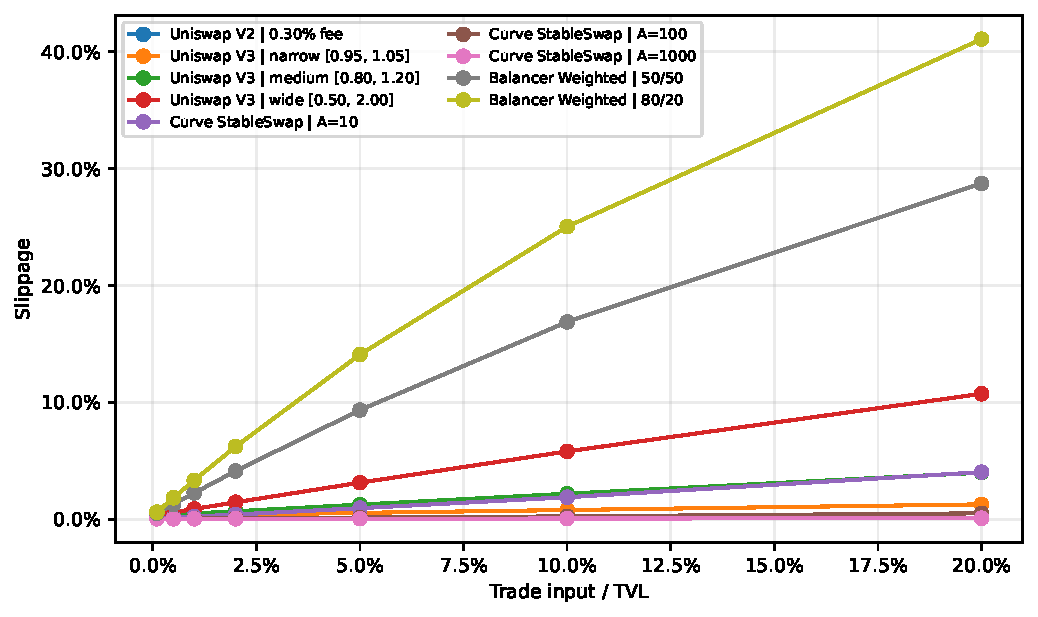
\includegraphics[width=\columnwidth]{slippage_comparison.pdf}
\caption{Slippage versus normalized trade size at \$1 million TVL.}
\label{fig:slippage}
\end{figure}

Figure~\ref{fig:slippage} shows that invariant choice strongly changes
execution. At a \pct{10}-of-TVL trade, V2 and Balancer 50/50 both produce
\pct{16.875} slippage, confirming their mathematical equivalence. Balancer
80/20 produces \pct{25.026} in the tested direction because token $x$ is
already the heavily weighted reserve; withdrawing token $y$ traverses a
steeper effective curve. Reversing direction would change this comparison, so
the result is not a general statement that 80/20 pools always have worse
execution.

V3 demonstrates the benefit of concentrating capital. At the same
\pct{10}-of-TVL input, narrow, medium, and wide ranges produce \pct{0.789},
\pct{2.179}, and \pct{5.802} slippage. Their advantage is conditional on the
trade remaining near the active interval. A sufficiently large input reaches
the lower bound, after which this single-position model supplies no additional
liquidity.

StableSwap is the most efficient around parity. At \pct{10} input, slippage
falls from \pct{1.883} at $A=10$ to \pct{0.246} at $A=100$ and \pct{0.061} at
$A=1000$. Increasing $A$ flattens the near-parity curve, but the later
impermanent-loss result shows why this efficiency is not free.

\begin{figure}[t]
\centering
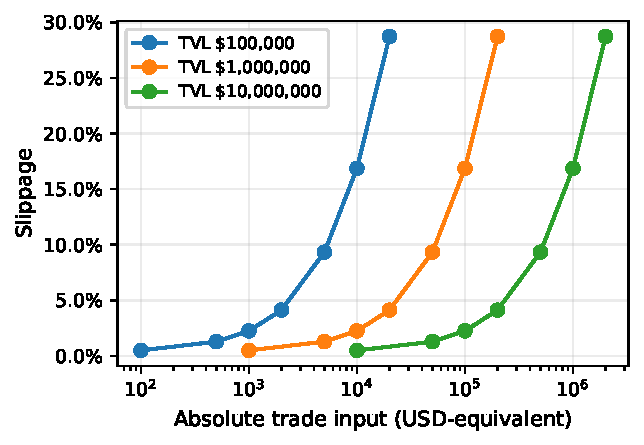
\includegraphics[width=\columnwidth]{liquidity_effect.pdf}
\caption{A fixed absolute trade receives lower V2 slippage as TVL increases.}
\label{fig:liquidity}
\end{figure}

Figure~\ref{fig:liquidity} separates normalized shape from absolute scale.
For a given trade/TVL ratio, constant-product slippage is identical across
liquidity levels. For a fixed dollar-equivalent trade, however, a larger pool
moves less because the trade represents a smaller reserve fraction. This
explains why ``high liquidity'' must be defined relative to intended order
size.

\begin{figure}[t]
\centering
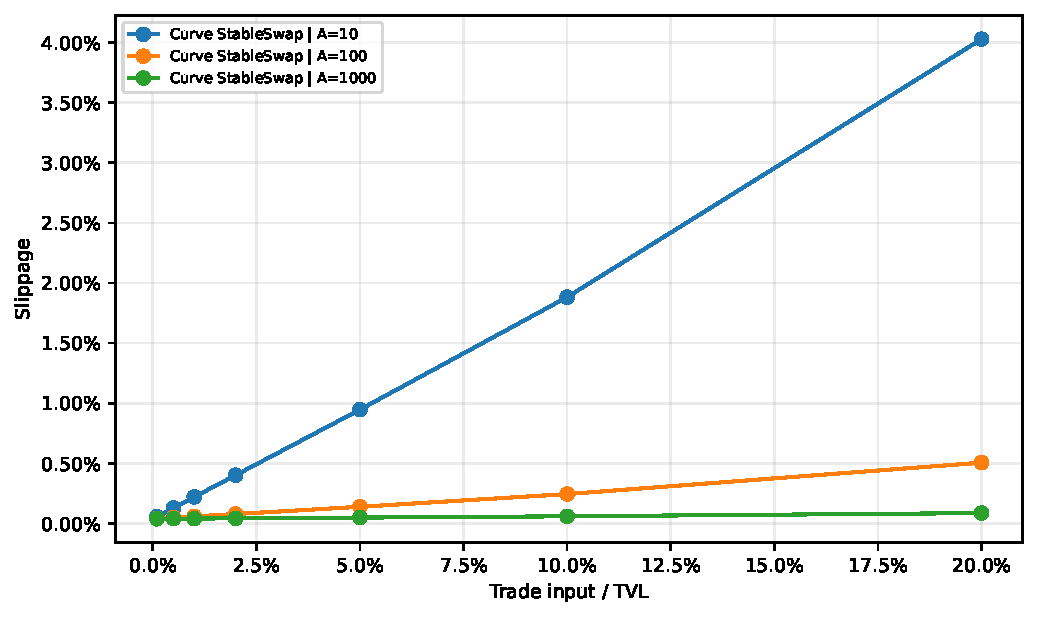
\includegraphics[width=\columnwidth]{stableswap_amplification.pdf}
\caption{Amplification reduces StableSwap slippage near parity.}
\label{fig:stable-slip}
\end{figure}

\clearpage
\section{Impermanent-Loss Results}

\begin{figure}[t]
\centering
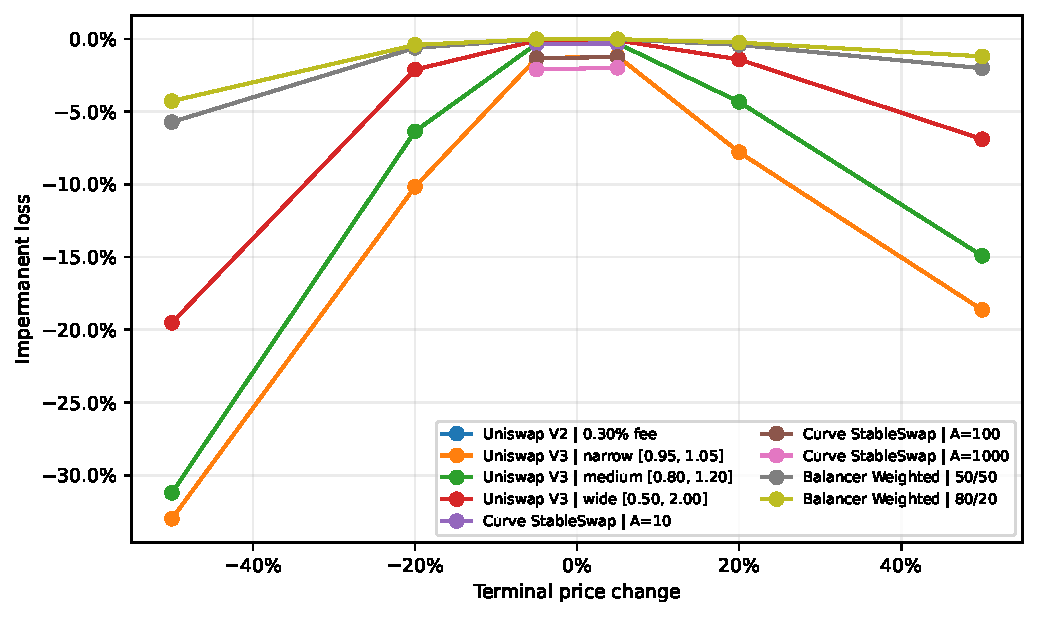
\includegraphics[width=\columnwidth]{impermanent_loss.pdf}
\caption{Impermanent loss relative to each configuration's initial holdings.}
\label{fig:il}
\end{figure}

Figure~\ref{fig:il} exposes the opposite side of capital efficiency. At a
$+\pct{50}$ terminal move, V2 and Balancer 50/50 lose \pct{2.020} relative to
holding. Balancer 80/20 loses \pct{1.203}, because its invariant trades less of
the initially dominant token for this direction and its benchmark preserves
the same 80/20 exposure. At $-\pct{50}$, the losses are larger:
\pct{5.719} for 50/50 and \pct{4.275} for 80/20. The asymmetry occurs because
equal percentage increases and decreases do not represent reciprocal prices.

Fixed-range V3 positions have much stronger range risk. At $+\pct{50}$,
narrow, medium, and wide positions lose \pct{18.635}, \pct{14.919}, and
\pct{6.898}. At $-\pct{50}$ the losses become \pct{32.998}, \pct{31.217}, and
\pct{19.526}. A narrow position exchanges its inventory aggressively inside a
small interval and then becomes entirely one token. Its superior local
liquidity therefore creates a larger opportunity cost when price leaves the
range.

StableSwap is shown only around parity. For a $+\pct{5}$ move, IL rises in
magnitude from \pct{0.311} at $A=10$ to \pct{1.245} at $A=100$ and
\pct{1.988} at $A=1000$. Strong amplification maintains a near-one internal
price longer, allowing arbitrageurs to remove more of the appreciating asset
during a depeg. High $A$ is appropriate only when the economic assumption of
correlation is credible.

\section{LP-Return Results}

\begin{figure}[t]
\centering
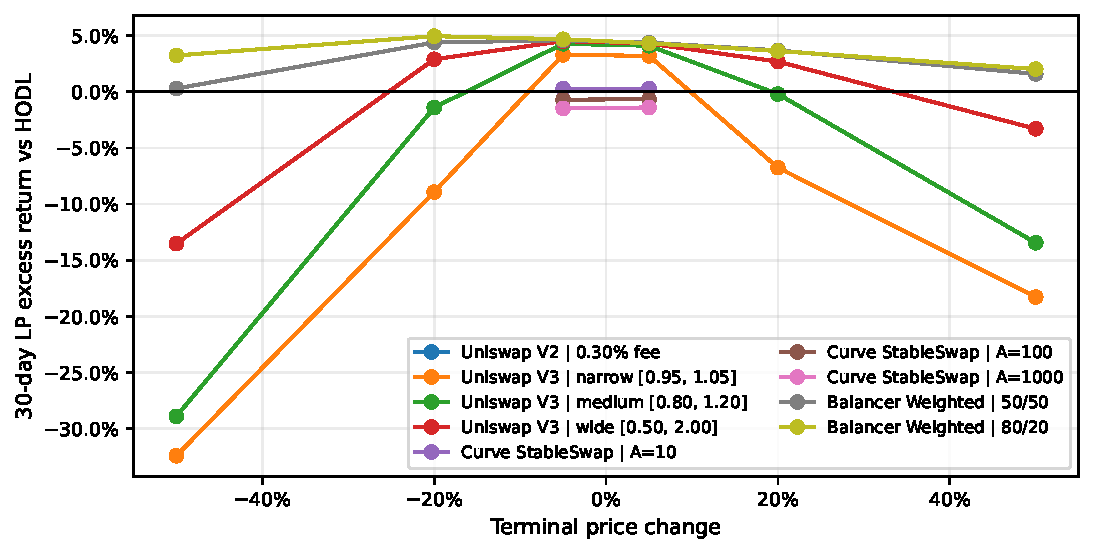
\includegraphics[width=\columnwidth]{lp_return.pdf}
\caption{Deterministic 30-day LP return at daily volume equal to \pct{50} of
TVL.}
\label{fig:return}
\end{figure}

At \pct{50} daily volume, a \pct{0.30} fee produces a gross 30-day fee return
of \pct{4.5} before V3 availability adjustment. This covers V2 IL for all
positive-price cases in the scenario set: net return is \pct{4.086} at
$+\pct{20}$ and \pct{2.480} at $+\pct{50}$. It does not cover the
$-\pct{50}$ stress case, where net return is $-\pct{1.219}$.

Balancer 80/20 has the highest net return among volatile-pair full-range models
in these tested directions because it receives the same assumed fee rate while
experiencing lower IL. Its net return is \pct{4.244} at $+\pct{20}$ and
\pct{3.297} at $+\pct{50}$. This conclusion depends directly on equal volume
and fee assumptions; actual order flow may differ by pool design.

V3 outcomes depend on both IL and time in range. At $+\pct{20}$, the wide
range earns \pct{3.086}, the medium range approximately breaks even at
\pct{0.165}, and the narrow range loses \pct{6.664}. The narrow range earns
fees for only one quarter of the assumed linear path before price crosses its
upper bound. The result demonstrates that headline capital efficiency is not
the same as realized LP return.

StableSwap charges only \pct{0.04} in this model, giving a \pct{0.6} gross
30-day fee return at \pct{50} daily volume. This covers the $A=10$ small-depeg
loss but not the $A=100$ or $A=1000$ loss. A highly amplified pool therefore
requires either stronger confidence in the peg, more volume, a higher fee, or
additional risk controls.

\section{Volume Sensitivity}

The fixed-volume scenarios make the break-even dependence explicit.
Table~\ref{tab:volume} reports net return at a $+\pct{20}$ terminal move. V2
and both weighted pools remain positive even at \pct{10} daily volume because
their IL is small in this scenario. The V3 wide position requires more than
\pct{10} daily volume to break even, while the medium position requires close
to the \pct{50} case. The narrow position remains negative even at daily volume
equal to TVL because it is active for only one quarter of the assumed price
path and its IL dominates collected fees.

\begin{table}[t]
\centering
\caption{30-day net return at $+\pct{20}$ price change.}
\label{tab:volume}
\small
\begin{tabular}{lrrr}
\toprule
Configuration & \pct{10} & \pct{50} & \pct{100}\\
\midrule
V2 / Weighted 50/50 & 0.49\% & 4.09\% & 8.59\%\\
Weighted 80/20 & 0.64\% & 4.24\% & 8.74\%\\
V3 narrow & -7.56\% & -6.66\% & -5.54\%\\
V3 medium & -3.44\% & 0.16\% & 4.66\%\\
V3 wide & -0.51\% & 3.09\% & 7.59\%\\
\bottomrule
\end{tabular}
\end{table}

Volume sensitivity also clarifies why the return analysis is not a forecast.
The simulator assigns the same volume fraction to mechanisms with very
different execution quality. In a real market, low slippage may attract more
flow, while fragmented liquidity, incentives, routing, and fee tiers determine
which LPs receive that flow. The controlled assumption is useful because it
isolates fee-rate and availability effects, but deployment analysis must
replace it with observed or modeled order flow.

\clearpage
\section{Mechanism Comparison and Market Fit}

\begin{table*}[t]
\centering
\caption{Qualitative interpretation of the simulated trade-offs.}
\small
\begin{tabular}{p{0.15\textwidth}p{0.18\textwidth}p{0.18\textwidth}p{0.19\textwidth}p{0.17\textwidth}}
\toprule
Mechanism & Main strength & Main LP risk & Suitable market & Important caveat\\
\midrule
V2 constant product & General, continuous full-range liquidity & IL under directional movement & Permissionless volatile pairs & Capital is spread over all prices\\
V3 fixed range & Very low local slippage & Range exit and one-sided inventory & Pairs with active LP management or bounded expectations & Fixed positions can stop earning fees\\
StableSwap & Extremely low near-parity slippage & Depeg drains the stronger asset & Credibly correlated or redeemable assets & Higher $A$ magnifies depeg exposure\\
Weighted pool & Encodes desired portfolio weights & Direction-dependent execution and IL & Treasury, index, and liquidity bootstrapping designs & Comparison must preserve weighted hold benchmark\\
\bottomrule
\end{tabular}
\end{table*}

No configuration dominates every metric. StableSwap and narrow V3 both
increase local capital efficiency by making stronger assumptions about where
price should remain. StableSwap assumes correlation; V3 LPs choose a bounded
interval. When those assumptions fail, inventory changes more aggressively
than in a general full-range pool.

V2 is comparatively inefficient for small trades because liquidity is spread
from zero to infinity, but it is robust in the limited sense that liquidity
never becomes inactive. Its simple invariant also provides a transparent
baseline for auditing other designs. Balancer extends this baseline by
allowing the pool itself to represent a portfolio preference. That can reduce
IL relative to the corresponding weighted hold position, but it changes
directional depth and should not be judged with a 50/50 benchmark.

For traders, the relevant question is whether active liquidity exists for the
intended trade and direction. For LPs, the relevant question is whether fee
income compensates for inventory rebalancing under plausible price paths.
These perspectives can conflict: the configuration offering traders the least
slippage can expose LPs to the strongest adverse selection.

\section{Limitations}

The simulator is deliberately deterministic. Its results should be interpreted
as controlled mechanism comparisons, not forecasts.

\begin{itemize}
  \item Fee income is proportional to an assumed daily volume and does not
  model endogenous volume, fee compounding, or competition among LPs.
  \item Terminal IL is path independent for the full-range analytical models,
  while actual fee earnings and V3 inventory management are path dependent.
  \item V3 uses one fixed position and a linear-path availability factor. It
  excludes ticks shared by other LPs, active repositioning, gas, and
  rebalancing losses.
  \item StableSwap uses two equally valued assets and an ideal arbitrage
  equilibrium. It excludes admin fees, imbalance fees, withdrawal behavior,
  and irreversible depeg dynamics.
  \item Balancer tests token $x$ input only. Weighted pools have intentionally
  asymmetric depth, so reverse-direction execution must be evaluated
  separately for a deployment decision.
  \item Smart-contract precision, integer rounding, oracle behavior, gas, and
  protocol-specific implementation details are outside the analytical model.
\end{itemize}

These limits are also why the report avoids a single ``best AMM'' score.
Combining metrics into one number would require subjective probabilities for
volume, volatility, depeg, range management, and trade direction.

\section{Reproducibility and Validation}

The implementation separates invariant modules from shared metrics and
experiment orchestration. Automated tests cover known outputs, invariant
preservation, V3 inventory below/inside/above its range, StableSwap
amplification behavior, zero-change IL, deterministic scenario counts, and
figure generation. The approved YAML configuration expands to 189 slippage
rows, 42 IL rows, and 126 LP-return rows.

The experiment command regenerates all CSV files and PDF figures. No random
number generator or external API is used. This makes every table and figure
repeatable from the repository state and allows individual assumptions to be
changed without rewriting model code.

\begin{table}[t]
\centering
\caption{Selected validation claims and automated checks.}
\small
\begin{tabular}{p{0.43\columnwidth}p{0.47\columnwidth}}
\toprule
Claim & Check\\
\midrule
V2 and weighted 50/50 are equivalent & Equal output and invariant tests\\
Swaps remain on their invariant & Pre/post numerical tolerance tests\\
V3 becomes one-sided outside range & Below, inside, and above inventory tests\\
Higher $A$ reduces near-parity slippage & Ordered quote comparison\\
IL uses the correct hold benchmark & Zero-change and known V2 formula tests\\
Experiments are reproducible & Exact row counts and deterministic frames\\
\bottomrule
\end{tabular}
\end{table}

Reproduction requires three commands from the repository root: run
\texttt{pytest}; run \texttt{scripts/run\_experiments.py} with
\texttt{PYTHONPATH=src}; then compile \texttt{report/main.tex} with Tectonic.
Generated CSV files remain available for auditing values that are summarized
or rounded in this report.

\section{Conclusion}

AMM design shifts risk rather than eliminating it. Constant product offers a
general full-range baseline but produces material slippage for large reserve
fractions. Concentrated liquidity improves execution dramatically near the
current price, at the cost of strong range-dependent LP outcomes. StableSwap
achieves the lowest near-parity slippage in the study, but high amplification
turns a small depeg into a meaningful LP loss. Weighted pools preserve
asymmetric portfolio exposure and can reduce IL relative to that weighted
benchmark, while producing direction-dependent execution.

For general volatile markets without active LP management, V2-like full-range
liquidity remains the simplest robust choice. For bounded or actively managed
markets, V3 can use capital much more efficiently. For credibly redeemable or
correlated assets, StableSwap offers superior execution when amplification is
selected conservatively. Weighted pools are most useful when portfolio
exposure is itself part of the protocol objective. The appropriate mechanism
therefore follows from market assumptions, LP objectives, and acceptable
failure modes.

\begin{thebibliography}{9}
\bibitem{univ2}
H. Adams, N. Zinsmeister, and D. Robinson,
\emph{Uniswap v2 Core}, 2020.
\url{https://app.uniswap.org/whitepaper.pdf}

\bibitem{univ3}
H. Adams et al.,
\emph{Uniswap v3 Core}, 2021.
\url{https://app.uniswap.org/whitepaper-v3.pdf}

\bibitem{curve}
M. Egorov,
\emph{StableSwap: Efficient Mechanism for Stablecoin Liquidity}, 2019.
\url{https://docs.curve.finance/references/whitepaper}

\bibitem{balancer}
F. Martinelli and N. Mushegian,
\emph{A Non-Custodial Portfolio Manager, Liquidity Provider, and Price Sensor},
2019.
\url{https://balancer.fi/whitepaper.pdf}
\end{thebibliography}

\end{document}
